\renewcommand{\theequation}{\theenumi}
\begin{enumerate}[label=\arabic*.,ref=\thesubsection.\theenumi]
\numberwithin{equation}{enumi}
\item
The signal constellation for binary frequency shift keying (BFSK) is given in Fig. \ref{fig:bfsk_const}.
Obtain the equations for the received symbols.

\begin{figure}[!h]
\centering
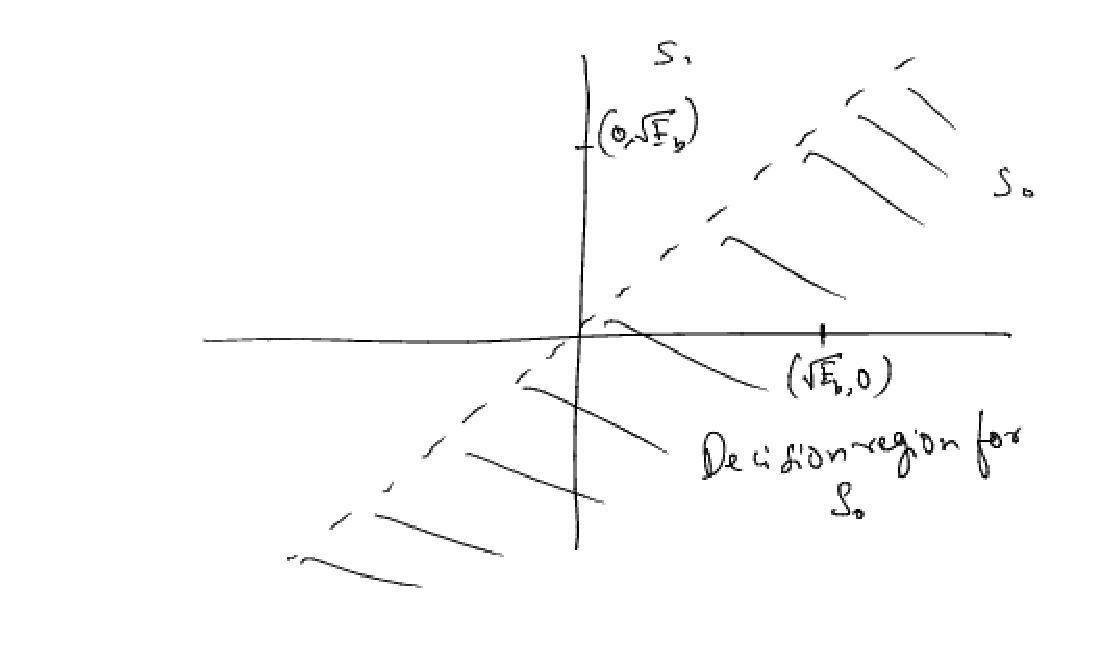
\includegraphics[width=\columnwidth]{./modulation/manual/figs/bfsk_const.eps}
\caption{}
\label{fig:bfsk_const}
\end{figure}
\solution
The received symbols are given by
\begin{align}
\mathbf{y}|s_0 = 
\begin{pmatrix*}
\sqrt{E_b} \\
0
\end{pmatrix*}
+
\begin{pmatrix*}
 n_{1}\\
n_{2}
\end{pmatrix*},
\end{align}
and 
\begin{align}
\mathbf{y}|s_1 = 
\begin{pmatrix*}
0\\
\sqrt{E_b} 
\end{pmatrix*}
+
\begin{pmatrix*}
n_{1}\\
 n_{2}
\end{pmatrix*},
\end{align}
where $n_1,n_2 \sim \gauss{0}{\frac{N_0}{2}}$. and
$
\mathbf{y} = 
\begin{pmatrix*}
y_{1}\\
 y_{2}
\end{pmatrix*}
$.
\item
Obtain a decision rule for BFSK from Fig. \ref{fig:bfsk_const}.

\solution The decision rule is
\begin{equation}
\label{eq:bfsk_dec}
y_1 \dec{s_0}{s_1} y_2
\end{equation}
%The multivariate Gaussian distribution is defined as
%%
%\begin{multline}
%p_{\mathbf{x}}(x_1,\dots,x_k)
%\\
%=\frac{1}{\sqrt{\brak{2\pi}^k\abs{\Sigma}}}\exp\cbrak{-\frac{1}{2}\brak{\mathbf{x}-\mathbf{\mu}}^T\Sigma^{-1}\brak{\mathbf{x}-\mathbf{\mu}}}
%\end{multline}
%%
%where $\mathbf{\mu}$ is the mean vector, $\Sigma = E\sbrak{\brak{\mathbf{x}-\mathbf{\mu}}\brak{\mathbf{x}-\mathbf{\mu}}^T}$ is the covariance matrix and $\abs{\Sigma}$ is the determinant of $\Sigma$.
\begin{definition}
The joint PDF of $X,Y$ is given by
\begin{multline}
\label{eq:bivariate}
p(x,y)= \frac{1}{2\pi \sigma_x\sigma_y\sqrt{1-\rho^2}}\exp\lsbrak{-\frac{1}{2\brak{1-\rho^2}}}
\\
\times \rsbrak{\cbrak{\frac{\brak{x-\mu_x}^2}{\sigma_x^2}+\frac{\brak{y-\mu_y}^2}{\sigma_y^2}-\frac{2\rho\brak{x-\mu_x}\brak{y-\mu_y}}{\sigma_x\sigma_y}}}
\end{multline}
%
where
\begin{align}
\mu_x &= E\sbrak{X},
\sigma_x^2 = \text{var}\brak{X},
\rho = \frac{E\sbrak{\brak{X - \mu_x}\brak{Y-\mu_y}}}{\sigma_x\sigma_y}.
\end{align}
%where
%%
%\begin{align}
%\mathbf{\mu}=
%\begin{pmatrix*}
%\mu_x \\
%\mu_y
%\end{pmatrix*},
%\Sigma = 
%\begin{pmatrix*}%[r]
%\sigma_x^2 & \rho\sigma_x\sigma_y \\
%\rho\sigma_x\sigma_y & \sigma_y^2
%\end{pmatrix*}
%\end{align}
%
\end{definition}
%
\item
For equiprobably symbols, the MAP criterion is defined as
%
\begin{equation}
\label{eq:map_bfsk_dec}
p\brak{\mathbf{y}|s_0} \dec{s_0}{s_1} p\brak{\mathbf{y}|s_1}
\end{equation}
Use \eqref{eq:bivariate} in \eqref{eq:map_bfsk_dec}  to obtain \eqref{eq:bfsk_dec}.

\solution According to the MAP criterion, assuming equiprobably symbols,
\begin{align}
%\pr{ \mathbf{y}|s_0 }
p\brak{\mathbf{y}|s_0} \dec{s_0}{s_1} p\brak{\mathbf{y}|s_1}
\end{align}
\item
Derive and plot the probability of error.  Verify through simulation.

\solution Given that $s_0$ was transmitted, the received symbols are
\begin{align}
\mathbf{y}|s_0 = 
\begin{pmatrix*}
\sqrt{E_b} \\
0
\end{pmatrix*}
+
\begin{pmatrix*}
 n_{1}\\
n_{2}
\end{pmatrix*},
\end{align}
From \eqref{eq:bfsk_dec}, 
the probability of error is given by
\begin{align}
P_e &= \pr{y_1 < y_2|s_0} = \pr{\sqrt{E_b} + n_1 < n_2}
\\
&= \pr{ n_2-n_1 > \sqrt{E_b} } 
\label{eq:bfsk_proof_n0}
\end{align}
Note that $n_2-n_1 \sim \gauss{0}{N_0}$. Thus, 
\begin{align}
P_e &= \pr{ \sqrt{N_0}w > \sqrt{E_b} }  =  \pr{ w > \sqrt{\frac{E_b}{N_0}} }
%= \pr{ X > \sqrt{E_b} }
\\
\implies 
P_e & = \qfunc{\sqrt{\frac{E_b}{N_0}}}
\end{align}
where 
%$X \sim \gauss{0}{N_0}$
%\\
$w \sim \gauss{0}{1}$.  
%Then $X = \sqrt{N_0}w$. Substituting this in \eqref{eq:fsk_proof_n0},
%where $\qfunc{x} \define \pr{w > x}, x \ge 0$.
%
The following code plots the BER curves in Fig. \ref{fig:bfsk_ber}
\begin{lstlisting}
codes/modulation/fsk_ber.py
\end{lstlisting}
%
\begin{figure}[!h]
\centering
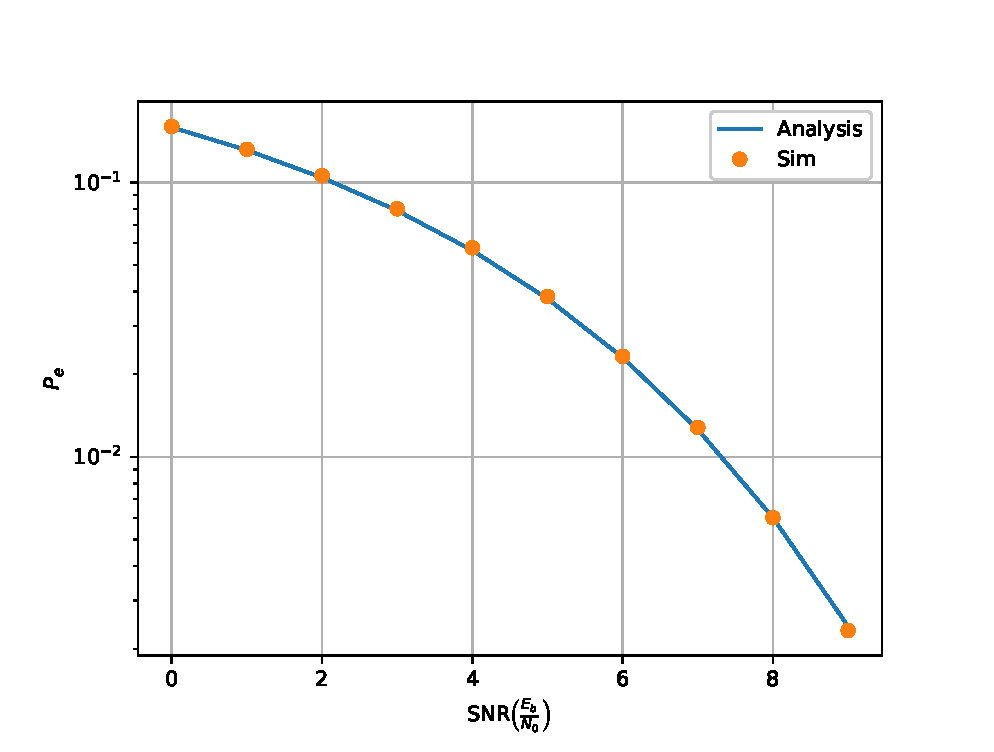
\includegraphics[width=\columnwidth]{./modulation/manual/figs/bfsk_ber.eps}
\caption{}
\label{fig:bfsk_ber}
\end{figure}
\end{enumerate}

